\section{LFSR as PRNG} \label{LFSR}
In this section we explain how CC2538 uses the CRC16 LFSR as a PRNG. 

\begin{figure}[!t]
\centering
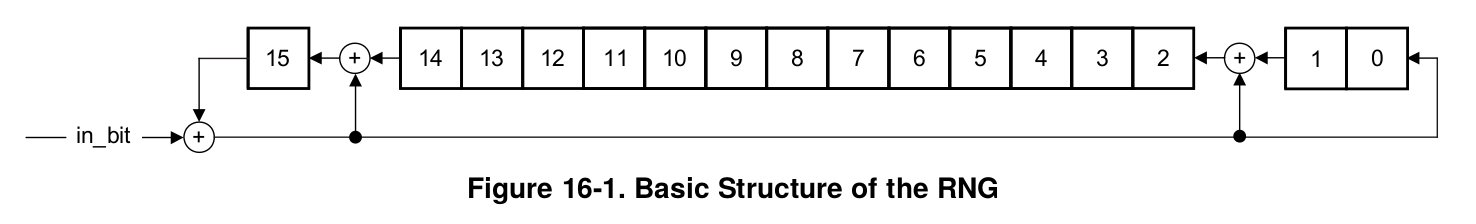
\includegraphics[width=2.5in]{fig/crc16.png}
\caption{CRC16 LFSR, from CC2538 User's Guide}
\label{CRC16}
\end{figure}

CC2538 User's Guide describes the PRNG design as: (Section 16.1 in CC2538 User's Guide)
\begin{quote}
The random-number generator is a 16-bit linear-feedback shift register (LFSR) with polynomial X 16 + X 15 +
X 2 + 1 (that is, CRC16). It uses different levels of unrolling depending on the operation it performs. The basic version (no unrolling) is shown in Figure 16-1 (\Cref{CRC16} in this paper).
\end{quote}

When used as a PRNG, the in\_bit of \Cref{CRC16} is constantly $0$. The Contiki driver calls the PRNG by: (Section 16.2.1in CC2538 User's Guide)
\begin{quote}
Another way to update the LFSR is to set the RCTRL bits in the SOC\_ADC\_ADCCON1 register to 01. This clocks the LFSR once (13x unrolling), and the RCTRL bits in the SOC\_ADC\_ADCCON1 register automatically clear when the operation completes.
\end{quote}

In another word, the LFSR is updated by performing 13 CRC16 operations in \Cref{CRC16}.

By nature, the LFSR based PRNG is stateful. Further more, the CRC16 operation is deterministic. Combined with the small space of $16$ bits, the output of PRNG can be easily predicted.

Since there are only 16 bits in the LFSR, we can denote the universal set of its  possible values $\mathbb{S}$ as:
\begin{equation} \label{PRNGState}
\mathbb{S} = \{ S_{i} | S_{i} \in \{2\}^{16}\}
\end{equation}
\Cref{PRNGState} also implies that the LFSR can have no more than $|\mathbb{S}| = 2^{16} = 65536$ values.

We also denote the LFSR update operation as:
\begin{equation}
F:\mathbb{S} \rightarrow \mathbb{S}
\end{equation}
where $F$ is $13$ times of the deterministic CRC16 operation.

Denote the random seed sampled by the radio noise as $S^*$. The PRNG can be formalised as:
\begin{equation}
	\begin{aligned}
	S_{0} &= S^* \\
	S_{i+1} &= F(S_{i})
	\end{aligned}
\end{equation}

Since ${S}$ is finite and $F$ is deterministic, the random number sequence will eventually results into a cyclic sequence. The maximum non-repetitive PRNG output sequence $R$ can be represented as:
\begin{equation}
R_{S^*}= (F^0(S^{*}), F^{1}(S^{*}), ..., F^{n-2}(S^{*}, F^{n-1}(S^{*}))
\end{equation}
where $S^{*} = F^{0}(S^{*}) = F^{n}(S^{*})$. Since the sequence is non-repetitive, we have $n \leq |\mathbb{S}|$. In another word, the cycle of PRNG output can be no longer than $65536$ calls.

A property of the sequence is that if a re-sampled seed $S^{*'}$ has appeared in $R_{S^*}$, i.e. $S^{*'} = F^{k}(S^*)$ where $k \in \mathbb{Z}_n$, then its corresponding maximum non-repetitive PRNG output sequence will be:
\begin{equation}
	\begin{aligned}
	R_{S^{*'}} = &( F^{k}(S^*), F^{k+1}(S^{*}), ..., F^{n-1}(S^*), F^{0}(S^*), ...,\\
	&F^{k-2}(S^{*}), F^{k-1}(S^{*})
	\end{aligned}
\end{equation}

That is to say $R_{S^{*'}}$ can be obtained through cyclic left rotating $R_{S^*}$ by $k$ times. As a result, assume consecutive calls to the PRNG seeded by $S^*$ generated a random number sequence $R_0$ such that:
\begin{equation}
R_0 = (S_i, S_{i+1}, ..., S_{j})
\end{equation}

Then $R_0$ will definitely be reproduced during consecutive calls to the PRNG seeded by seed $S^{*'}$ as well. This property can be exploited to completely break DTLS as we will explain in \Cref{BreakDTLS}.

This property also indicates that if a seed that is not inside $R_{S^*}$, denote as $S^{**} \notin R_{S^*}$, then there will be no over lapped elements between  $R_{S^{**}}$ and  $R_{S^{**}}$.

By enumerating the 16 bit space of $\mathbb{S}$, our experiment on CC2538 has shown that for CC2538 PRNG there exists four non-overlapping sequence(source code available at \cite{prngtest}):
\begin{itemize}
	\item $R_{0x0001}$ with $n = 32766$.
	\item $R_{0x0003}$ with $n = 32767$.
	\item $R_{0x0000}$ with $n = 1$.
	\item $R_{0x8003}$ with $n = 1$.
\end{itemize}
where $R_{0x0000}$ and $R_{0x8003}$ are excluded by the manual\cite{CC2538Manual}.

The enumeration can be done within a few minutes. Any other sequences can be transformed to the above sequences through cyclic left rotation. 

\section{Breaking DTLS} \label{BreakDTLS}
tinydtls\cite{tinydtls} is a DTLS implementation on Contiki. Its current available version\cite{tinydtls082} (0.8.2) supports two cipher suites, namely Pre Shared Key (PSK) and ECDHE\_ECDSA\cite{rfc4492}. The only curve supported by the implementation is secp256r1\cite{secp256r1}.

As explained in \Cref{LFSR}, the CC2538 PRNG output is a predictable stream of cycle less than $2^{16}$ calls; therefore the possible key selection can be easily enumerated and leads to a complete break of cryptographic systems relies on its randomness.    

\Cref{KeyGen} briefly describes the ECC Key Generation.
\begin{figure}
	\begin{algorithmic}[1]
	\scriptsize
	\REQUIRE Domain Parameter $T = (p, a, b, G, n, h)$ as specified by \cite{secp256r1}.
	\STATE Randomly select $d \in [1, n-1]$.
	\STATE Compute $Q = dG$.
	\RETURN $(Q,d)$, where $Q$ is the public key and $d$ the secret key.
	\end{algorithmic}
	\caption{ECC Key Generation}
	\label{KeyGen}
\end{figure}

tinydtls does not have its own RNG implementation; instead it invokes the Contiki system RNG API random\_rand(), of which output is predictable, in a loop to generate arbitrary length of random number (tinydlts/dtls\_prng.h). Since $T$ is public, this vulnerability would allow an adversary to pre-compute the public keys by enumerating all secret keys beginning in each position of $R_{0x0000}$ and $R_{0x0001}$ and build up a look up table. Upon observing a public key, the adversary can immediately invert its corresponding secret key in the table.

We have generated such a look up table in \cite{prngtest}. The pre-computation for the $65536$ keys takes less than 5 minutes on a laptop powered by i7-2620M. 
The attack can be applied to two targets during a DTLS handshake of ECDHE\_ECDSA.

\begin{itemize}
\item \paragraph{\textbf{ECDHE}}
	\begin{figure}
		\begin{algorithmic}[1]
		\scriptsize
		\REQUIRE Domain Parameter $T = (p, a, b, G, n, h)$. Party $A$'s key pair $(Q_A, d_A)$ and party $B$'s key pair $(Q_B, d_B)$. 
		\STATE $A$ randomly picks $r_A \in [0, n-1]$. 
		\STATE $B$ randomly picks $r_B \in [0, n-1]$.
		\STATE $A$ computes $Q_A = {r_A}G$ and sends $Q_A$ to $B$.
		\STATE $B$ computes $Q_B = {r_B}G$ and sends $Q_B$ to $A$.
		\STATE Both $A$ and $B$ computes $Q_{AB} = {r_A}{r_B}G = {r_A}{Q_B} = {r_B}{Q_A}$.
		\RETURN Both $A$ and $B$ returns $K = Hash(Q_{AB})$ as the shared secret.
		\end{algorithmic}
		\caption{ECDHE}
		\label{ECDHE}
	\end{figure}
	
	ECDHE is a key exchange protocol that allows two party to derive a shared secret. In DTLS, ECDHE is performed at the end of DTLS handshake to derive a shared symmetric key that is used for encrypting data packets. \Cref{ECDHE} provides a brief description of ECDHE. The adversary can recover $r_A$ and $r_B$ by observing $Q_A$ and $Q_B$ that is being sent in the packets; hence computes $K$ to derive the symmetric key used in later communication.

\item \paragraph{\textbf{ECDSA}}
	\begin{figure}
		\begin{algorithmic}[1]
		\scriptsize
		\REQUIRE Domain Parameter $T = (p, a, b, G, n, h)$, server key pair $(Q,d)$ and a message to be signed $m$.
		\STATE Randomly select $k \in [1, n-1]]$.
		\STATE Compute $kG = (x_1, y_1)$ and let $r = x_1 \mod n$.
		\STATE Compute $e = SHA-1(m)$.
		\STATE Compute $s = k^{-1}(e + dr) \mod n$.
		\RETURN $(m,r,s)$ as the message-signature pair.
		\end{algorithmic}
		\caption{ECDSA Signing}
		\label{ECDSA}
	\end{figure}
	
	ECDSA is an authentication scheme that allows a party to authenticate a message. In DTLS, it is used to sign the server parameters (details in \cite{rfc3279}) during the handshake to provide server authenticity. \Cref{ECDSA} briefly describes the signing scheme of ECDSA. The adversary observing $(m,r,s)$ can revert $k$ by searching $r$ in the look up table. He can then recover the server secret key $d$ by computing:
	\begin{equation}
		\begin{aligned}
		e &= SHA-1(m) \\
		d &= r^{-1}(sk - e) \mod n
		\end{aligned}
	\end{equation}
	With the knowledge of $k$, the adversary will be able to impersonate the victim server.
\end{itemize}

We have tested the attacks by sniffing two CC2538 nodes performing handshake using the example code provided by tinydtls. The secret keys have been successfully recovered using the look up table in \cite{prngtest}.

\section{Reflection on PRNG design}
%Stdlib implementation
Investigating RNG implementations in other platforms supported by Contiki, we realised that most of them does not have a dedicated RNG implementation and by default wraps rand() in stdlib as the RNG. Hence we investigated the some of the open sourced stdlib implementations. For the majority, i.e. stdlib for ARM\cite{ARMrand}, AVR\cite{AVRrand} and MSP430\cite{MSP430rand}, the rand() implementation can be abstracted as \Cref{rand}. The type of variable \textit{seed}  may vary on different platforms. The \textit{do\_rand()} function outputs a congruent of linear transformation of \textit{seed} before updates it.
 
\begin{figure}
\lstinputlisting[breaklines=true,basicstyle=\scriptsize]{src/rand.c}
\caption{rand() implementations in stdlib}
\label{rand}
\end{figure}

It is clear that such design would also yield into a predictable random number stream with cycle no longer than the range of \textit{seed}, as the same \textit{seed} will return the same output. On the above platforms, the cycles are no longer than are $2^{32}$, $2^{16}$ and $2^{16}$ respectively.

%Improvements (NIST 800-90A)
As an improvement, we suggest to use more sophisticated PRNG implementation for cryptographic applications. \cite{NISTPRNG} has recommended several PRNG constructions based on approved hash functions and block ciphers. Specifically for CC2538, SHA-256 and AES have hardware coprocessor support and hence can be considered candidates for implementing cryptographically secure PRNG according to \cite{NISTPRNG}.



